\documentclass[polish,12pt]{article}
\usepackage[T1]{fontenc}
\usepackage[utf8]{inputenc}
\usepackage{babel}
\usepackage{a4wide}
\usepackage{geometry}
\geometry{verbose,a4paper,tmargin=3cm,bmargin=3cm,lmargin=2.5cm,rmargin=2.5cm}
\usepackage{epsfig}
\usepackage{pslatex}
\usepackage{setspace}

\begin{document}
\thispagestyle{empty}
~
\vspace{8em}
~
\begin{center}
  
\epsfig{file=surealived-logo.eps, width=8cm}
\end{center}
\begin{center}
  \textbf{\Large Moduły testujące}\\
  \vspace{2em}
  \large
  Zbigniew Kempczyński\\
  Bartosz Ponurkiewicz
\end{center}
\newpage

\tableofcontents
\newpage

\section{Pisanie własnego modułu}
Moduły testujące (zwane dalej \textit{testerami}) udostępniają \textbf{surealived} funkcje
które następnie są wywoływane przez surealived według następującego schematu:
\begin{center}
  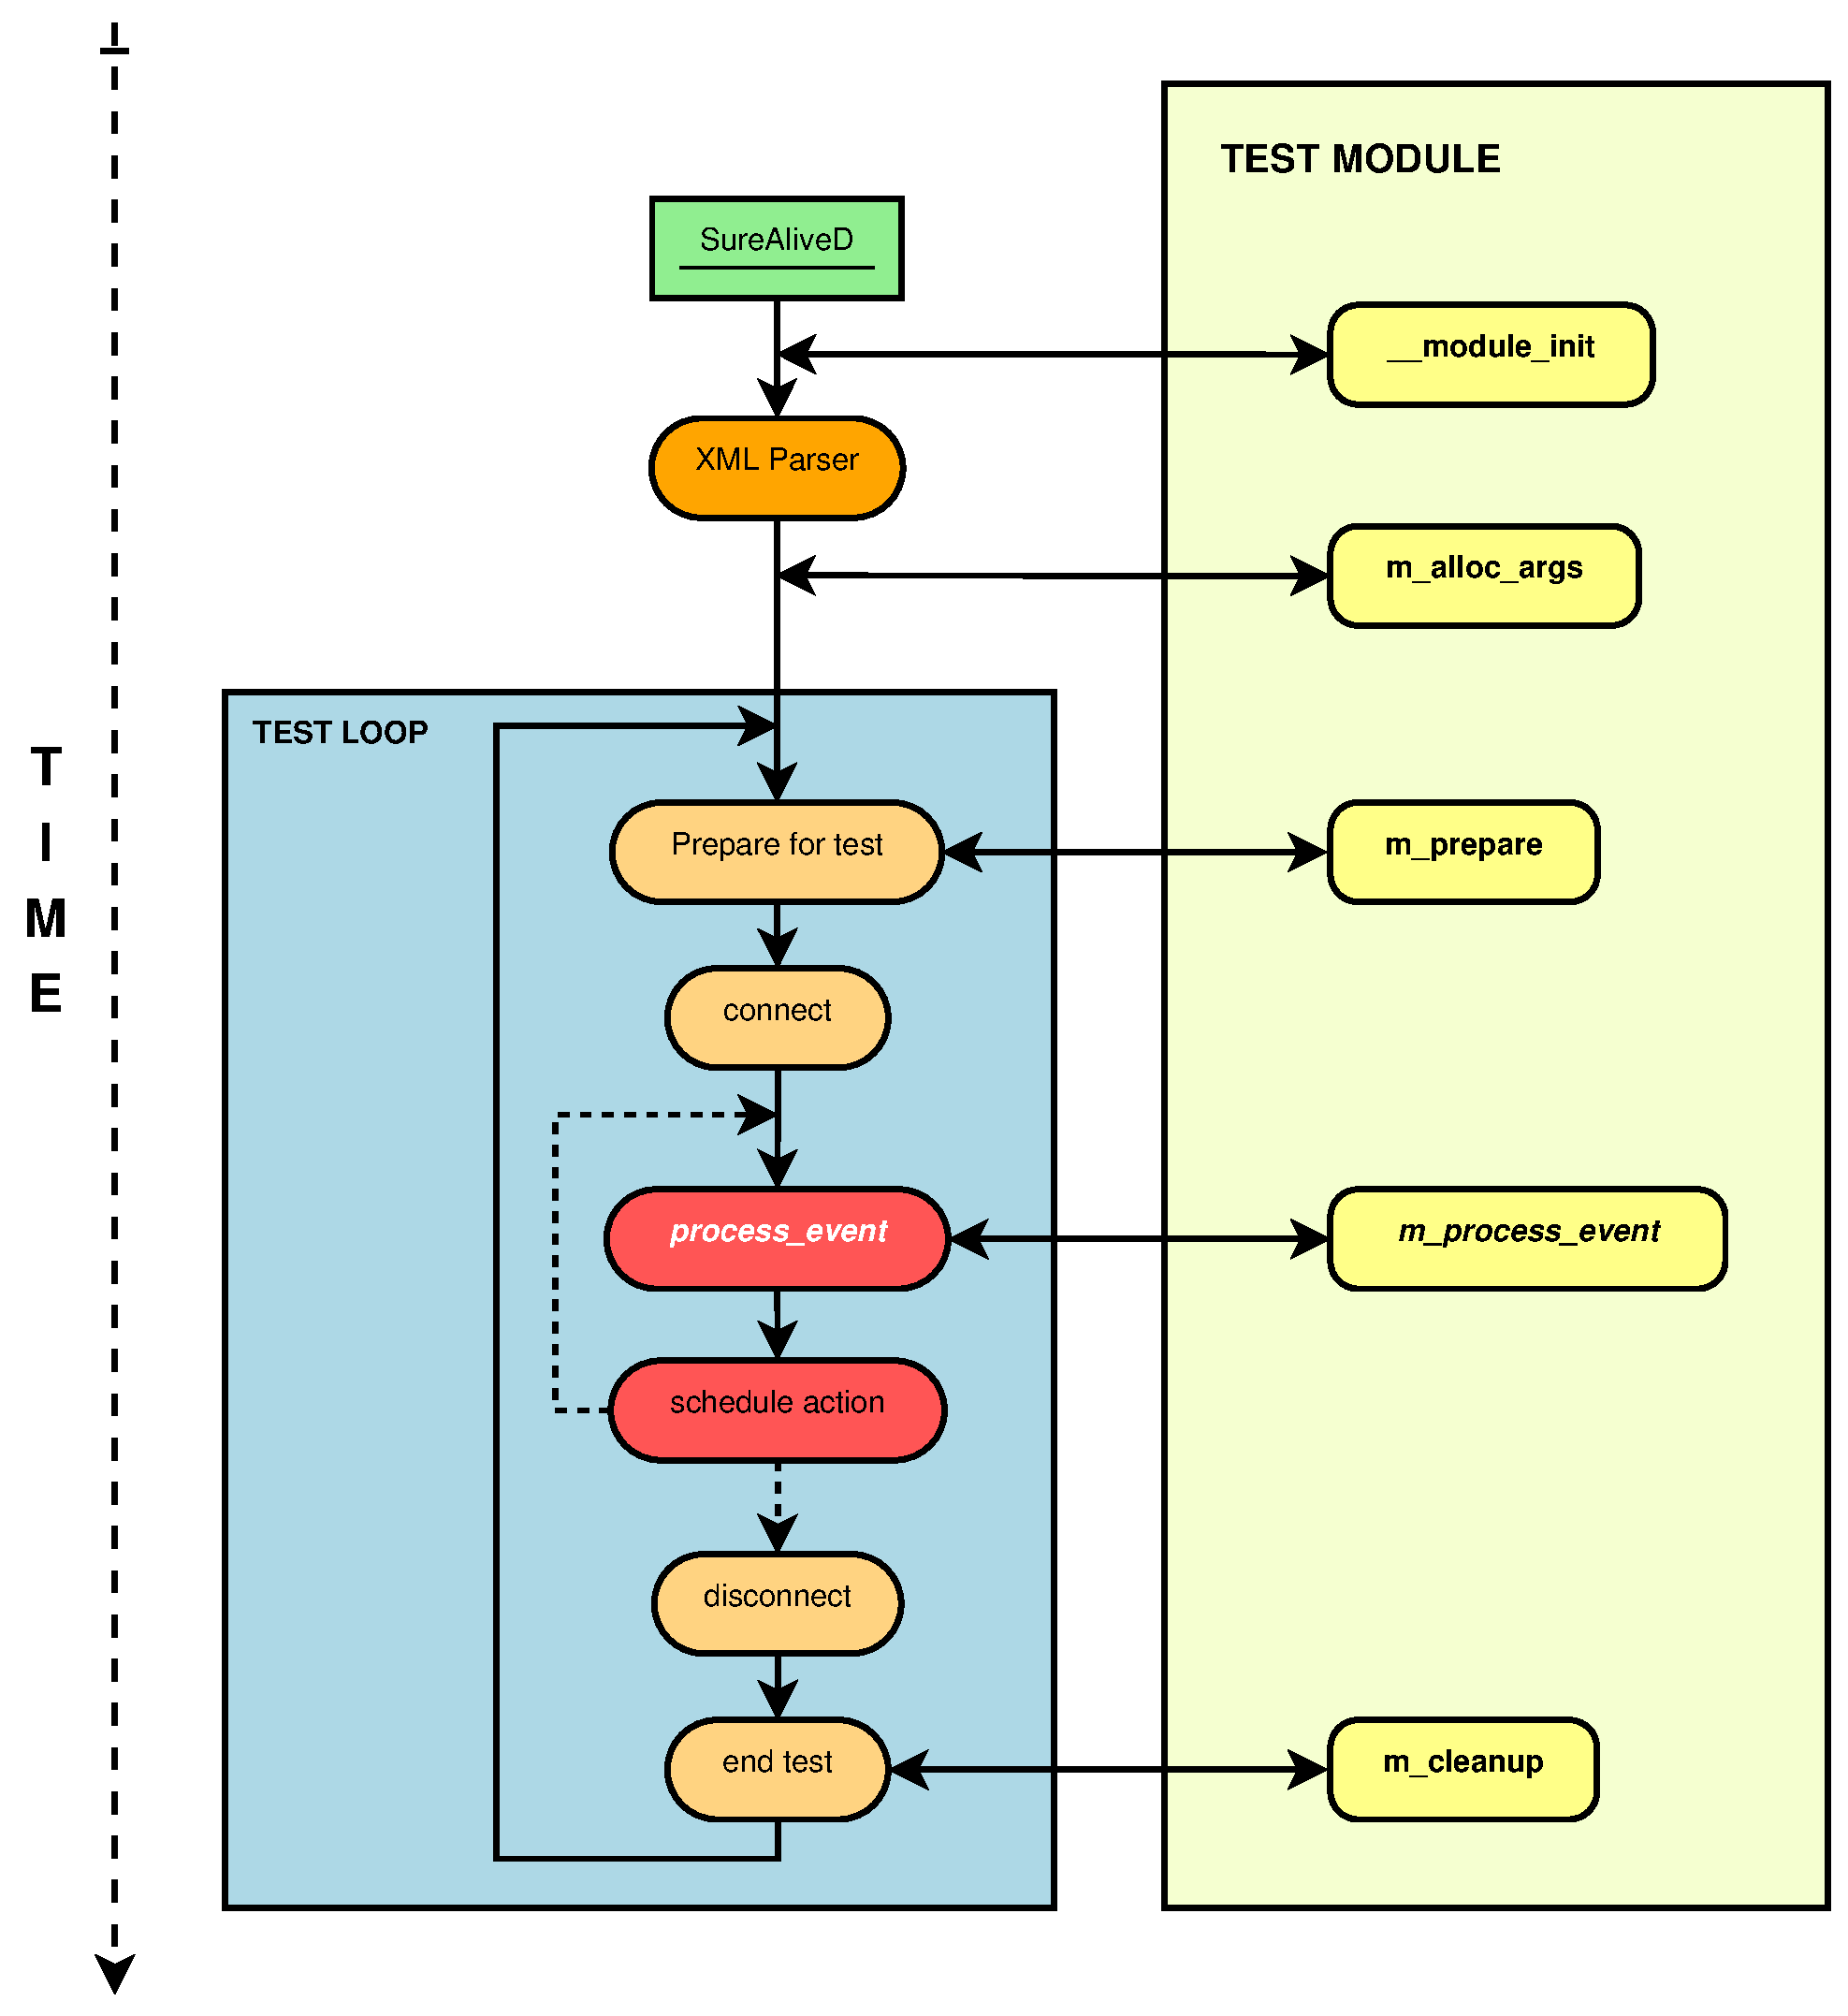
\epsfig{file=module_flow.eps, width=16cm}
\end{center}

\newpage

\subsection{Informacje o module}
Moduł musi przedstawić się w grzeczny sposób \textbf{surealived}, w tym celu konieczne
jest, aby zadeklarował i uzupełnił strukturę typu \textbf{mod\_operations}:
{\small
\begin{verbatim}
typedef struct mod_operations {
    gpointer        (*m_alloc_args)(void);
    void            (*m_free)(CfgReal *); /* free all real's memory */
    void            (*m_prepare)(CfgReal *);
    void            (*m_cleanup)(CfgReal *);
    REQUEST         (*m_process_event)(CfgReal *);
    void            (*m_check)(CfgReal *); /* exec */
    void            (*m_start)(CfgReal *); /* exec */
    gchar           *m_name;
    mod_args        *m_args;
    SDTestProtocol  m_test_protocol;
} mod_operations;
\end{verbatim}
}
Opis pól struktury:
\begin{itemize}
  \item \textbf{m\_alloc\_args} -- wskaźnik na funkcję zwracającą wskaźnik na strukturę
    prywatnych danych \textit{reala}
  \item \textbf{m\_free} -- wskaźnik na funkcję zwalniającą pamięć podczas usuwania \textit{reala}
    z konfiguracji (np podczas odpinania serwera)
  \item \textbf{m\_prepare} -- wskaźnik na funkcję inicjującą test \textit{reala}
  \item \textbf{m\_cleanup} -- wskaźnik na funkcję sprzątającą po teście
  \item \textbf{m\_process\_event} -- wskaźnik funkcji obsługującej przychodzące zdarzenia
  \item \textbf{m\_start}/\textbf{m\_check} -- funkcje wykorzystywane przez mod\_exec
  \item \textbf{m\_name} -- nazwa modułu
  \item \textbf{m\_args} -- wskaźnik na tablicę struktur \textit{mod\_args}
  \item \textbf{m\_test\_protocol} -- typ używanego protokołu do komunikacji,
    \newline
    możliwe wartości to \textbf{SD\_PROTO\_(TCP|UDP|EXEC|NO\_TEST)}

\end{itemize}
\newpage
\subsection{Inicjalizacja}
Podczas ładowania modułu \textbf{SureAliveD} wywołuje jego funkcję inicjalizującą, która zwraca
strukturę typu \textit{mod\_args}. Funkcja inicjalizująca moduł \textbf{MUSI} nazywać się
\textbf{\_\_init\_module}. Przykładowa implementacja tej funkcji w module wygląda tak:
{\small
\begin{verbatim}
static mod_operations mops;   /* Module operations struct */

mod_operations __init_module(void) {
    mops.m_name             = "http";
    mops.m_test_protocol    = SD_PROTO_TCP;
    mops.m_args             = m_args;

    mops.m_alloc_args       = module_alloc_args;
    mops.m_prepare          = module_test_prepare;
    mops.m_process_event    = module_process_event;
    mops.m_free             = module_free;
    return mops;
}
\end{verbatim}
}
\subsection{Parametry własne modułu (per real)}
Konfiguracja \textbf{SureAliveD} odnośnie testowanych usług znajduje się w pliku XML.
W tym pliku można definiować dodatkowe parametry które mają sterować pracą modułów testujących.
Moduł musi więc w jakiś sposób informować \textbf{surealived} o parametrach jakich oczekuje
podczas konfiguracji. Przede wszystkim musi on stworzyć strukturę jaka będzie definiować
możliwe zmienne.
{\small
\begin{verbatim}
typedef struct {
    char        url[BUFSIZ];
    char        host[256];
    char        *request;
    int         req_len;
    bool        naive;
} TestHTTP;
\end{verbatim}
}
\newpage
Oprócz tego moduł musi stworzyć tablicę struktur typu \textbf{mod\_args}, zakończoną NULL'em,
która opisuje strukturę zmiennych używanych przez moduł. Dzięki strukturze \textit{mod\_args}
\textbf{surealived} będzie wiedział jak rozparsować konfigurację XML.
{\small
\begin{verbatim}
typedef struct {
    gchar           *name;        /* attribute name */
    SD_MODARG_TYPE  type;         /* type (STRING/INT/...) */
    guint           param;        /* optional parameter (default value or length) */
    SD_ATTR_TYPE    attr_type;    /* BASIC_ATTR (necessary) or EXTRA_ATTR */
    unsigned long   offset;       /* Use SDOFF makro to define offset */
} mod_args;
\end{verbatim}
}
\begin{itemize}
  \item \textit{name} -- określa nazwę atrybutu w konfiguracji XML.
  \item \textit{type} -- typ argumentu, możliwe typy to: \textbf{STRING, PORT, UINT, INT, BOOL}
  \item \textit{param} -- określa maksymalną długość dla STRING lub domyślną wartość dla innych typów.
  \item \textit{attr\_type} -- określa czy argument jest konieczny do konfiguracji czy też dodatkowy.
  \item \textit{offset} -- przesunięcie zmiennej względem struktury w której się znajduje, tutaj najlepiej
    jest użyć makra SDOFF podając jako pierwszy argument nazwę struktury a jako drugi nazwę zmiennej.
\end{itemize}
Na przykład:
{\small
\begin{verbatim}
static mod_args m_args[]={
    { "url",     STRING,    BUFSIZ, BASIC_ATTR, SDOFF(TestHTTP, url)     },
    { "host",    STRING,    256,    BASIC_ATTR, SDOFF(TestHTTP, host)    },
    { "naive",   BOOL,      -1,     EXTRA_ATTR, SDOFF(TestHTTP, naive)   },
    { "retcode", INT,       200,    EXTRA_ATTR, SDOFF(TestHTTP, retcode) },
    { NULL, 0,  0,  0,  0 },
};
\end{verbatim}
}
Nie jest konieczne definiowanie wszystkich zmiennych zawartych w strukturze,
nie będą one jednak ustawiane podczas parsowania (mogą służyć jako dane prywatne \textit{reala}).\\
Ważne jest natomiast, aby tablica była zakończona NULL'em.
\newline
Rolą modułu jest alokacja pamięci potrzebnej na strukturę atrybutów, w tym celu \textbf{surealived}
wywołuje funkcję \textit{m\_alloc\_args} zadeklarowaną w strukturze \textit{mod\_operations}.
Przykładowa funkcja \textit{m\_alloc\_args}:
{\small
\begin{verbatim}
static gpointer module_alloc_args(void) {
    TestHTTP    *ret = g_new0(TestHTTP, 1);
    memset(ret, 0, sizeof(TestHTTP));
    return ret;
}
\end{verbatim}
}
Od tej pory ustawieniem parametrów i rozparsowaniem XML'a zajmie się \textbf{surealived}
a moduł ma pewność, że parametry będą ustawione zgodnie z tym co zdefiniował w tablicy
\textit{mod\_args}.

\subsection{Opis struktury CfgReal}
W kolejnych etapach modułu parametrem przekazywanym funkcjom obsługi testu przekazywany
jako parametr jest wskaźnik do struktury CfgReal. Oto opis najważniejszych pól tejże struktury:
\begin{itemize}
  \item \textbf{char *virt->name} -- nazwa \textit{virtuala} do którego podpięty jest \textit{real}
  \item \textbf{char *buf} -- wskaźnik na bufor do/z którego \textbf{surealived} ma wczytywać/zapisywać dane
  \item \textbf{gboolean test\_state} -- stan testu TRUE/FALSE
  \item \textbf{char error} -- zmienna określająca wystąpienie błędu w transmisji
  \item \textbf{u\_int32\_t bytes\_read} -- ilość przeczytanych bajtów w ostatniej operacji
  \item \textbf{u\_int32\_t intstate} -- stan \textit{reala} zmienna pomocna modułom
  \item \textbf{char name[MAXNAME]} -- nazwa \textit{reala}
  \item \textbf{char addrtxt[MAXIPTXT]} -- adres (w formacie czytelnym dla ludzi)
  \item \textbf{char porttxt[MAXPORTTXT]} -- port (w formacie czytelnym dla ludzi)
  \item \textbf{gpointer moddata} -- wskaźnik na strukturę zaalokowaną przez moduł dla konkretnego
    \textit{reala}
\end{itemize}

\subsection{Ustawianie parametrów testu}
Przed przystąpieniem do testu \textbf{SureAliveD} wywołuje funkcję \textit{m\_prepare} zdefiniowaną
w strukturze \textit{module\_operations}, jej zadaniem jest ustawienie odpowiednich wartości koniecznych
do przeprowadzenia testu (przede wszystkim ustawienia stanu testu). Jako parametr funkcja ta dostaje
wskaźnik na strukturę konfiguracyjną \textit{reala}.
\begin{verbatim}
static void m_prepare(CfgReal *real); /* definicja funkcji */
\end{verbatim}
Struktura \textit{CfgReal} zawiera m.in wskaźnik na strukturę prywatną \textit{reala} zdefiniowaną
przez moduł i zaalokowaną przez \textit{m\_alloc\_args}. Wskaźnik ten znajduje się w polu \textit{moddata}:
\begin{verbatim}
TestHTTP *t = (TestHTTP *)real->moddata;
\end{verbatim}

\newpage

\subsection{Obsługa zdarzeń testu}
\begin{verbatim}
REQUEST m_process_event(CfgReal *real)
\end{verbatim}
Funkcja \textit{m\_process\_event} wywoływana jest za każdym razem, gdy nadejdzie nowe zdarzenie dla
\textit{reala}.
\newline
Ewentualny błąd (np w wypadku zerwania połączenia) ustawiany jest w zmiennej \textit{real->error}.
Funkcja ta powinna implementować obsługę zdarzeń, musi też zwracać żądanie (\textbf{REQUEST})do \textbf{surealived}
możliwe żądania to:
\begin{itemize}
  \item \textbf{WANT\_READ(\textit{n})} -- żądanie odczytania DOKŁADNIE \textit{n} bajtów
  \item \textbf{WANT\_WRITE(\textit{n})} -- żądanie wysłania DOKŁADNIE \textit{n} bajtów
  \item \textbf{WANT\_READ\_AV(\textit{n})} -- żądanie odczytania NAJWYŻEJ \textit{n} bajtów, jednak moduł
    zostanie poinformowany po odebraniu pierwszego komunikatu
  \item \textbf{WANT\_EOF} -- moduł żąda poinformowania gdy na socket będzie pusty (brak danych),
    \newline wszystkie odczytane dane są tracone
  \item \textbf{WANT\_END} -- moduł zakończył testowanie i komunikację z realem należy zakończyć
\end{itemize}
\textit{\textbf{UWAGA!} W przypadku funkcji odczytujących/zapisujących wszystkie operacje
są wykonywane na wskaźniku \textit{buf} ze struktury CfgReal.
W intencji modułu jest ustawienie tego wskaźnika na poprawny obszar w pamięci.}

\subsection{Sprzątanie po teście}
\begin{verbatim}
void m_cleanup(CfgReal *real)
\end{verbatim}
Jeżeli przed lub w trakcie testu moduł zaalokował jakieś dane i nie będą one więcej wykorzystywane,
w tej właśnie funkcji należałoby zaalokowaną pamięć zwolnić. Funkcja \textit{m\_cleanup} jest 
wywoływana po zakończeniu testu.

\newpage
\subsection{Przykład}
W tym podrozdziale dokładnie przedstawimy sposób działania modułu \textit{mod\_http.c} testującego usługi
HTTP/HTTPS.
{\small
\begin{verbatim}
#include <stdio.h>
#include <glib.h>
#include <common.h>
#include <modloader.h>
#include <sd_defs.h>
#include <xmlparser.h>

#define REQUEST_TEMPLATE "GET %s HTTP/1.0\r\nHost: %s\r\nUser-Agent: SureAliveD\r\n\r\n"
\end{verbatim}
}
Podstawowe include'y z których najważniejsze (konieczne) są \textit{modloader.h}, \textit{sd\_defs.h} oraz
\textit{xmlparser.h} zawierają one definicje struktur i nazw.
REQUEST\_TEMPLATE zawiera ``szablon'' wysyłanego komunikatu (requestu) do serwera WWW.

\begin{verbatim}
typedef struct {
    gchar       url[BUFSIZ];
    gchar       host[256];
    gboolean    naive;
    gchar      *request;
    gint        req_len;
    gchar       ans[64];
    gchar       retcode[4];
} TestHTTP;

enum {
    CONNECTED,
    REQUEST_SENT,
    REQUEST_RECEIVED,
    RECEIVING
} State;
\end{verbatim}
Struktura TestHTTP zawiera informacje wykorzystywane przy teście.
State określa natomiast stan w jakim obecnie znajduje się \textit{real}
\newpage
{\small
\begin{verbatim}
static mod_operations mops;

static mod_args m_args[]={
    { "url",    STRING,     BUFSIZ, BASIC_ATTR, SDOFF(TestHTTP, url)    },
    { "host",   STRING,     256,    BASIC_ATTR, SDOFF(TestHTTP, host)   },
    { "naive",  BOOL,       -1,     EXTRA_ATTR, SDOFF(TestHTTP, naive)  },
    { "retcode", STRING,    4, EXTRA_ATTR, SDOFF(TestHTTP, retcode) },
    { NULL, 0,  0,  0,  0 },
};
\end{verbatim}
}
W tym miejscu następuje deklaracja struktury mod\_operations która zostanie wypełniona podczas inicjalizacji.
\newline
wypełniana jest też tablica m\_args[] zawierająca struktury typu mod\_args.
Witać wyraźnie, że od konfiguracji XML wymagamy dwóch parametrów obowiązkowych -- \textit{url}
typu STRING o maksymalnej długości BUFSIZ oraz \textit{host} o maksymalnej długości 256 bajtów.
Dodatkowe zmienne uwzględniane w konfiguracji to parametr \textit{naive} typu BOOL,
oraz \textit{retcode} określający oczekiwaną zwracaną wartość.
Ostatni element tablicy ``m\_args'' MUSI być wypełniony zerami.

\begin{verbatim}
static gpointer module_alloc_args(void) {
    TestHTTP    *ret = g_new0(TestHTTP, 1);
    memset(ret, 0, sizeof(TestHTTP));
    return ret;
}
\end{verbatim}
Funkcja \textit{module\_alloc\_args(void)} alokuje i wyzerowuje pamięć wielkości struktury TestHTTP
a następnie ją zwraca.
\newline
\newline
\begin{verbatim}
static void module_test_prepare(CfgReal *real) {
    TestHTTP    *t = (TestHTTP *)real->moddata;
    LOGDETAIL("http module test prepare");
    real->intstate = CONNECTED;
    if (!t->retcode[0])
        strncpy(t->retcode, "200", 3);
}
\end{verbatim}
Funkcja przygotowująca \textit{real} do testu, przede wszystkim ustawia stan (\textit{real->intstate})
na CONNECTED (ponieważ funkcja prepare jest wywoływana PO połączeniu) a następnie sprawdza czy podany
został alternatywny return code dla zapytania, jeżeli nie to ustawia standardowy ``HTTP \textbf{200} OK''
\newpage
\large \textbf{Faktyczna obsługa testu}\newline
\normalsize
{\small
\begin{verbatim}
static REQUEST module_process_event(CfgReal *real) {
    TestHTTP    *t = (TestHTTP *)real->moddata;

    if (real->error)
        return WANT_END;

    if (real->intstate == CONNECTED) {
        real->intstate = REQUEST_SENT;     /* set next state */

        real->buf = t->request;
        if (t->request)
            return WANT_WRITE(t->req_len);

        t->request = g_strdup_printf(REQUEST_TEMPLATE, t->url, t->host);

        real->buf  = t->request;
        t->req_len = strlen(t->request); /* and try to remember the length of it */

        LOGDETAIL("MOD_HTTP: requesting to write %d(%d) bytes",
                     t->req_len, REQ_LEN(WANT_WRITE(t->req_len)));
        return WANT_WRITE(t->req_len);
    }
\end{verbatim}
}
Początek funkcji obsługi zdarzeń sprawdza czy nie wystąpił błąd (zerwane połączenie) jeżeli tak, natychmiast
kończy test zwracająć żądanie WANT\_END.
\newline
Jeżeli jednak nie wystąpił błąd sprawdzany jest stan \textit{reala},
jeżeli dopiero nastąpiło połączenie (CONNECTED) moduł zmienia stan na REQUEST\_SENT i ustawia wskaźnik bufora
na prywatny bufor żądania dla \textit{reala} następnie sprawdza czy został już ustalony request dla reala,
jeżeli tak to żąda wysłania requestu do reala, jeżeli nie -- alokuje request podając potrzebne dane (url i host)
i zwraca żądanie zapisu.
\newline
{\small
\begin{verbatim}
    else if (real->intstate == REQUEST_SENT) {
        real->buf = t->ans;     /* drop answer to buf */
        memset(real->buf, 0, sizeof(t->ans));
        LOGDETAIL("MOD_HTTP: requesting to read %d(%d) bytes",
                     sizeof(t->ans), REQ_LEN(WANT_READ(sizeof(t->ans))));
        real->intstate = REQUEST_RECEIVED;
        return WANT_READ(sizeof(t->ans));
    }
\end{verbatim}
}
Jeżeli real znajduje się w stanie REQUEST\_SENT (dane zostały wysłane), to moduł zmienia bufor operacji
na prywatny bufor reala odpowiedzialny za trzymanie odpowiedzi, oraz zeruje pamięć w buforze.
Zmienia stan reala na REQUEST\_RECEIVED i zwraca żądanie odczytania dokładnie ``sizeof(t->ans)'' bajtów.
\newpage
{\small
\begin{verbatim}
    else if (real->intstate == REQUEST_RECEIVED) {
        if (!strncmp(real->buf+9, t->retcode, 3)) {
            LOGDETAIL("REAL ONLINE [virt:%s,%s]!", real->virt->name, real->name);
            real->test_state = TRUE;
        }
        else
            LOGDETAIL("REAL OFFLINE [virt:%s,%s]!", real->virt->name, real->name);

        if (t->naive)
            return WANT_END;

        real->intstate = EOF;
        return WANT_EOF;        /* notify me when you notice eof */
    }
    else {                      /* for statistics */
        LOGDETAIL("EOF on socket - statistics should be sent!");
    }
\end{verbatim}
}
Przedostatni możliwy stan testu to REQUEST\_RECEIVED, jeżeli real znajduje się w tym stanie,
następuje sprawdzenie poprawności ``return code'', jeżeli wszystko się zgadza moduł ustawia
stan testu (\textit{real->test\_state}) na TRUE. \newline
Następnie sprawdzany jest parametr \textit{naive} (podawany w XML'u), jeżeli został ustawiony
oznacza to, że w tym momencie należy zakończyć test, więc moduł zwraca żądanie zakończenia -- WANT\_END
w przeciwnym wypadku ustawiany jest stan testu na EOF i zwracane żądanie powiadomienia o końcu danych -- WANT\_EOF.
Funkcja \textit{module\_process\_event} zostanie uruchomiona gdy zakończy się odczyt wszystkich danych z socketu.
Przypadek ten zostanie obsłużony przez ostatniego ``else'a''.

\begin{verbatim}
static void module_free(CfgReal *real) {
    TestHTTP    *t = (TestHTTP *)real->moddata;
    if (t->request)
        free(t->request);
    t->request = NULL;
}
\end{verbatim}
Funkcja \textit{module\_free} zwalnia zaalokowaną pamięć. Funkcja ta wywoływana jest
w momencie usuwania reala z konfiguracji. NIE jest to funkcja m\_cleanup, która wywoływana
jest po zakończeniu każdego testu.
\newpage
{\small
\begin{verbatim}
mod_operations __init_module(void) {
    LOGINFO(" ** Init module: setting mod_operations for tester [http]");

    mops.m_name             = "http";
    mops.m_test_protocol    = SD_PROTO_TCP;
    mops.m_args             = m_args;

    mops.m_alloc_args       = module_alloc_args;
    mops.m_prepare          = module_test_prepare;
    mops.m_process_event    = module_process_event;
    mops.m_cleanup          = module_cleanup;
    return mops;
}
\end{verbatim}
}
Funkcja \textit{\_\_init\_module} inicjalizuje strukturę mod\_operations,
ustawia nazwę modułu, protokół komunikacji i strukturę zawierającą opis
argumentów przekazywanych modułowi. Ustawia też wskaźniki na funkcje obsługujące test
po czym zwraca strukturę do \textbf{surealived}.
Ta funkcja MUSI mieć dokładnie taką nazwę.

\section{Kompilacja modułu}
Moduł należy skompilować do postaci biblioteki współdzielonej. Można to zrobić np w ten sposób:
\begin{verbatim}
gcc -fPIC -shared -Wl,-soname,mod_NAME.so -o mod_NAME.so mod_NAME.c \
    `pkg-config --libs --cflags glib-2.0` `xml2-config --libs --cflags`
\end{verbatim}
Oczywiście należy zamienić mod\_NAME.so i mod\_NAME.c na nazwę modułu.
Należy przy tym pamiętać, aby podczas kompilacji dostępne były odpowiednie pliki nagłówkowe.
\end{document}
